\documentclass[a4,11pt]{aleph-notas}

% -- Paquetes adicionales
\usepackage{enumitem}
\usepackage{aleph-comandos}


% -- Datos   
\institucion{Escuela de Ciencias Físicas y Matemática}
\carrera{Ciencia de Datos}
\asignatura{Álgebra lineal}
\tema{Clase invertida no. 2: Aplicaciones Lineales}
\autor[A. Merino]{Andrés Merino}
\fecha{Semestre 2024-1}

\logouno[0.14\textwidth]{Logos/logoPUCE_04_ac}
\definecolor{colortext}{HTML}{0030A1}
\definecolor{colordef}{HTML}{0030A1}
\fuente{montserrat}

% -- Comandos adicionales
\begin{document}

\encabezado

\vspace*{-10mm}
\section*{Introducción}

\begin{itemize}
    \item \textbf{Tema:} Aplicaciones Lineales
    \item \textbf{Resultado de Aprendizaje:} Determina si una función es aplicación lineal o no.
\end{itemize}

\section*{Lección en casa}

\subsection*{Actividades}

\begin{enumerate}[leftmargin=*]
    \item Interactuar con ChatGPT mediante los siguientes \textit{prompts}, leyendo detenidamente el \textit{prompt} y su respuesta:
    \begin{enumerate}[label=\textit{Prompt \arabic*.},leftmargin=2.1cm]
        \item Vas a ser mi profesor de la asignatura de Álgebra Lineal, te iré dando indicaciones y me irás explicando de manera formal y luego de manera intuitiva los conceptos. Vas a tener mucho cuidado al escribir la parte matemática para que se visualice bien. Sé divertido. ¿Entendido?
        \item ¿Qué es una Aplicación Lineal?
        \item ¿Cómo se comprueba si una función es una aplicación lineal? No me des un ejemplo aún.
        \item Dame un ejemplo concreto en R2.
        \item Dame un ejemplo de algo que no sea aplicación lineal.
        \item Dame un ejemplo de aplicación lineal de R2 a R3.
        \item Dame un ejemplo de aplicación lineal de matrices de 2 por 2 a R3.
        \item Dame un ejemplo de aplicación lineal de R3 a matrices de 2 por 2.
        \item Plantéame dos funciones, una que sí sea aplicación lineal y otra que no, pero no me digas cuál es para ver si comprendí el concepto.
    \end{enumerate}
    \item Continuar la interacción hasta que te sientas preparado en el entendimiento del concepto.
    \item Copiar el enlace del chat como evidencia del proceso (ver Anexo).
    \item En caso de tener dudas sobre el tema, interactúa con tus compañeros de clase para solventarlas.
    \item Realiza el cuestionario del aula virtual.
\end{enumerate}

\section*{Anexo}

\subsection*{¿Cómo obtener el enlace de una conversación con ChatGPT?}

Seguir los siguientes pasos:
\begin{enumerate}
    \item Dar clic en los tres puntos a lado del nombre de la conversación.
    \item Seleccionar «Compartir».
    \begin{center}
        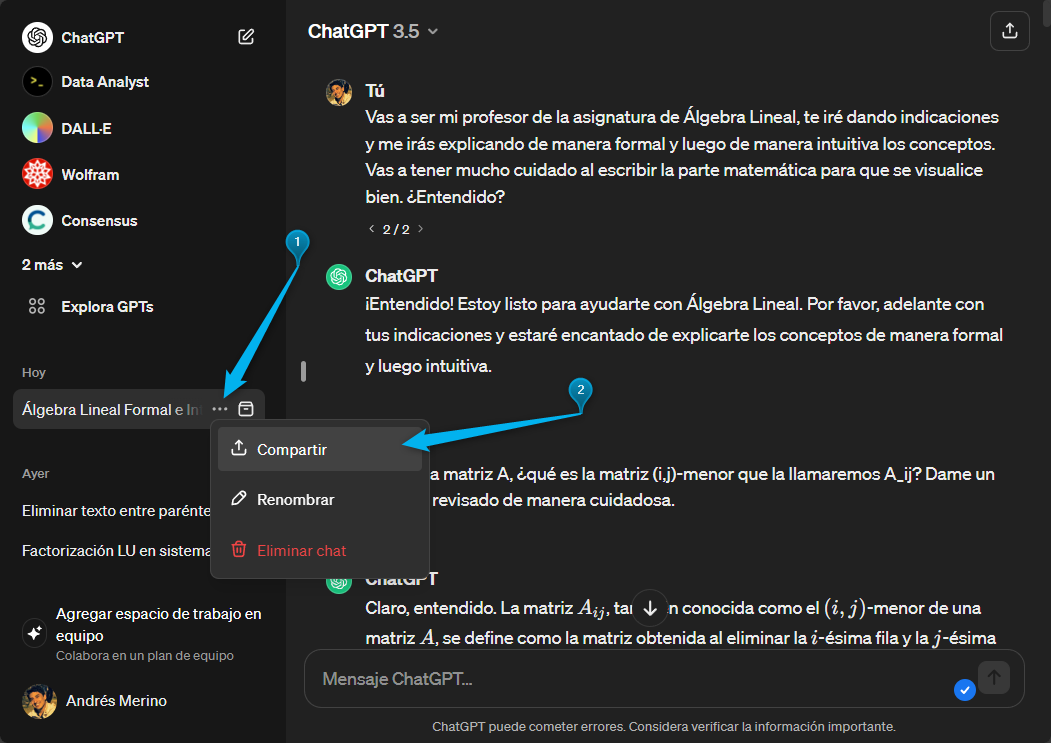
\includegraphics[width=0.85\linewidth]{Figuras/fig01.png}
    \end{center}
    \item En la nueva ventana, dar clic en los tres puntos. 
    \item Seleccionar «Compartir tu nombre».
    \item Dar clic en «Compartir enlace».

    \begin{center}
        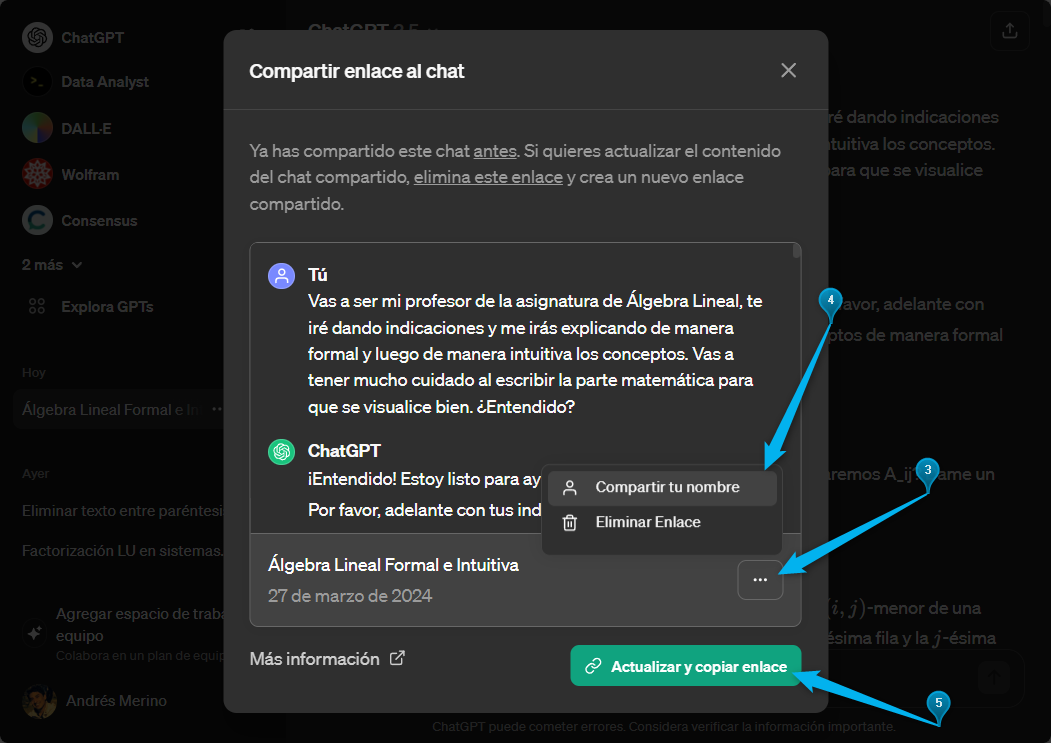
\includegraphics[width=0.85\linewidth]{Figuras/fig02.png}
    \end{center}
\end{enumerate}


\end{document}